
\documentclass[11pt]{article}
\usepackage[a4paper,margin=1in]{geometry}
\usepackage{amsmath,amssymb,amsthm,mathtools}
\usepackage{graphicx,booktabs}
\usepackage{hyperref}
\usepackage{cite}
\hypersetup{colorlinks=true, linkcolor=blue, urlcolor=blue, citecolor=blue}

\newtheorem{lemma}{Lemma}
\newtheorem{proposition}{Proposition}
\theoremstyle{remark}
\newtheorem{remark}{Remark}

\title{NB/BD Stability with M\"obius Weights:\\ Hutch++ Operator Control, PCG Implementation, and Contradiction Auto-Report}
\author{Serabi \\ Independent Researcher \\ \texttt{24ping@naver.com}}
\date{2025}

\begin{document}\maketitle

\begin{abstract}
We add Hutch++-based operator tracking for $\|E\|$, a diagonal+band preconditioned conjugate gradient (PCG) implementation, and an automatic contradiction reporter that cross-checks persistent residuals against operator growth. The pipeline reads CSV logs and regenerates plots.
\end{abstract}

\section{Operator Control via Hutch++}
With matvec oracles for $E$ and $E^\top$, we estimate ${\rm tr}(E^\top E)$ using Hutch++; the bound $\|E\|\le\sqrt{{\rm tr}(E^\top E)}$ monitors far-band leakage. The sketch size $(s,r)$ trades variance and cost.

\section{PCG with Diagonal+Band Preconditioner}
We solve normal equations with PCG and $P=\mathrm{diag}(A)+\mathrm{band}_k(A)$; $k=3$ works well in our tests. This reduces iteration counts roughly by a factor of $\log N$ at large scales.

\section{Contradiction Auto-Report}
We declare a ``persistence event'' if recent $d_N$ exceed $\varepsilon_0$ while the fitted $\theta$ falls below $\theta_{\min}$; if simultaneously Hutch++ shows bounded $\|E\|$, the event conflicts with bandwise decay and triggers a contradiction flag.

\section{Reproducibility}
Results are logged in \texttt{data/results\_v28.csv}. Figures are regenerated by \texttt{code/plot\_update.py}. Reports are produced by \texttt{code/contradiction\_report.py}.

\begin{figure}[h]
\centering
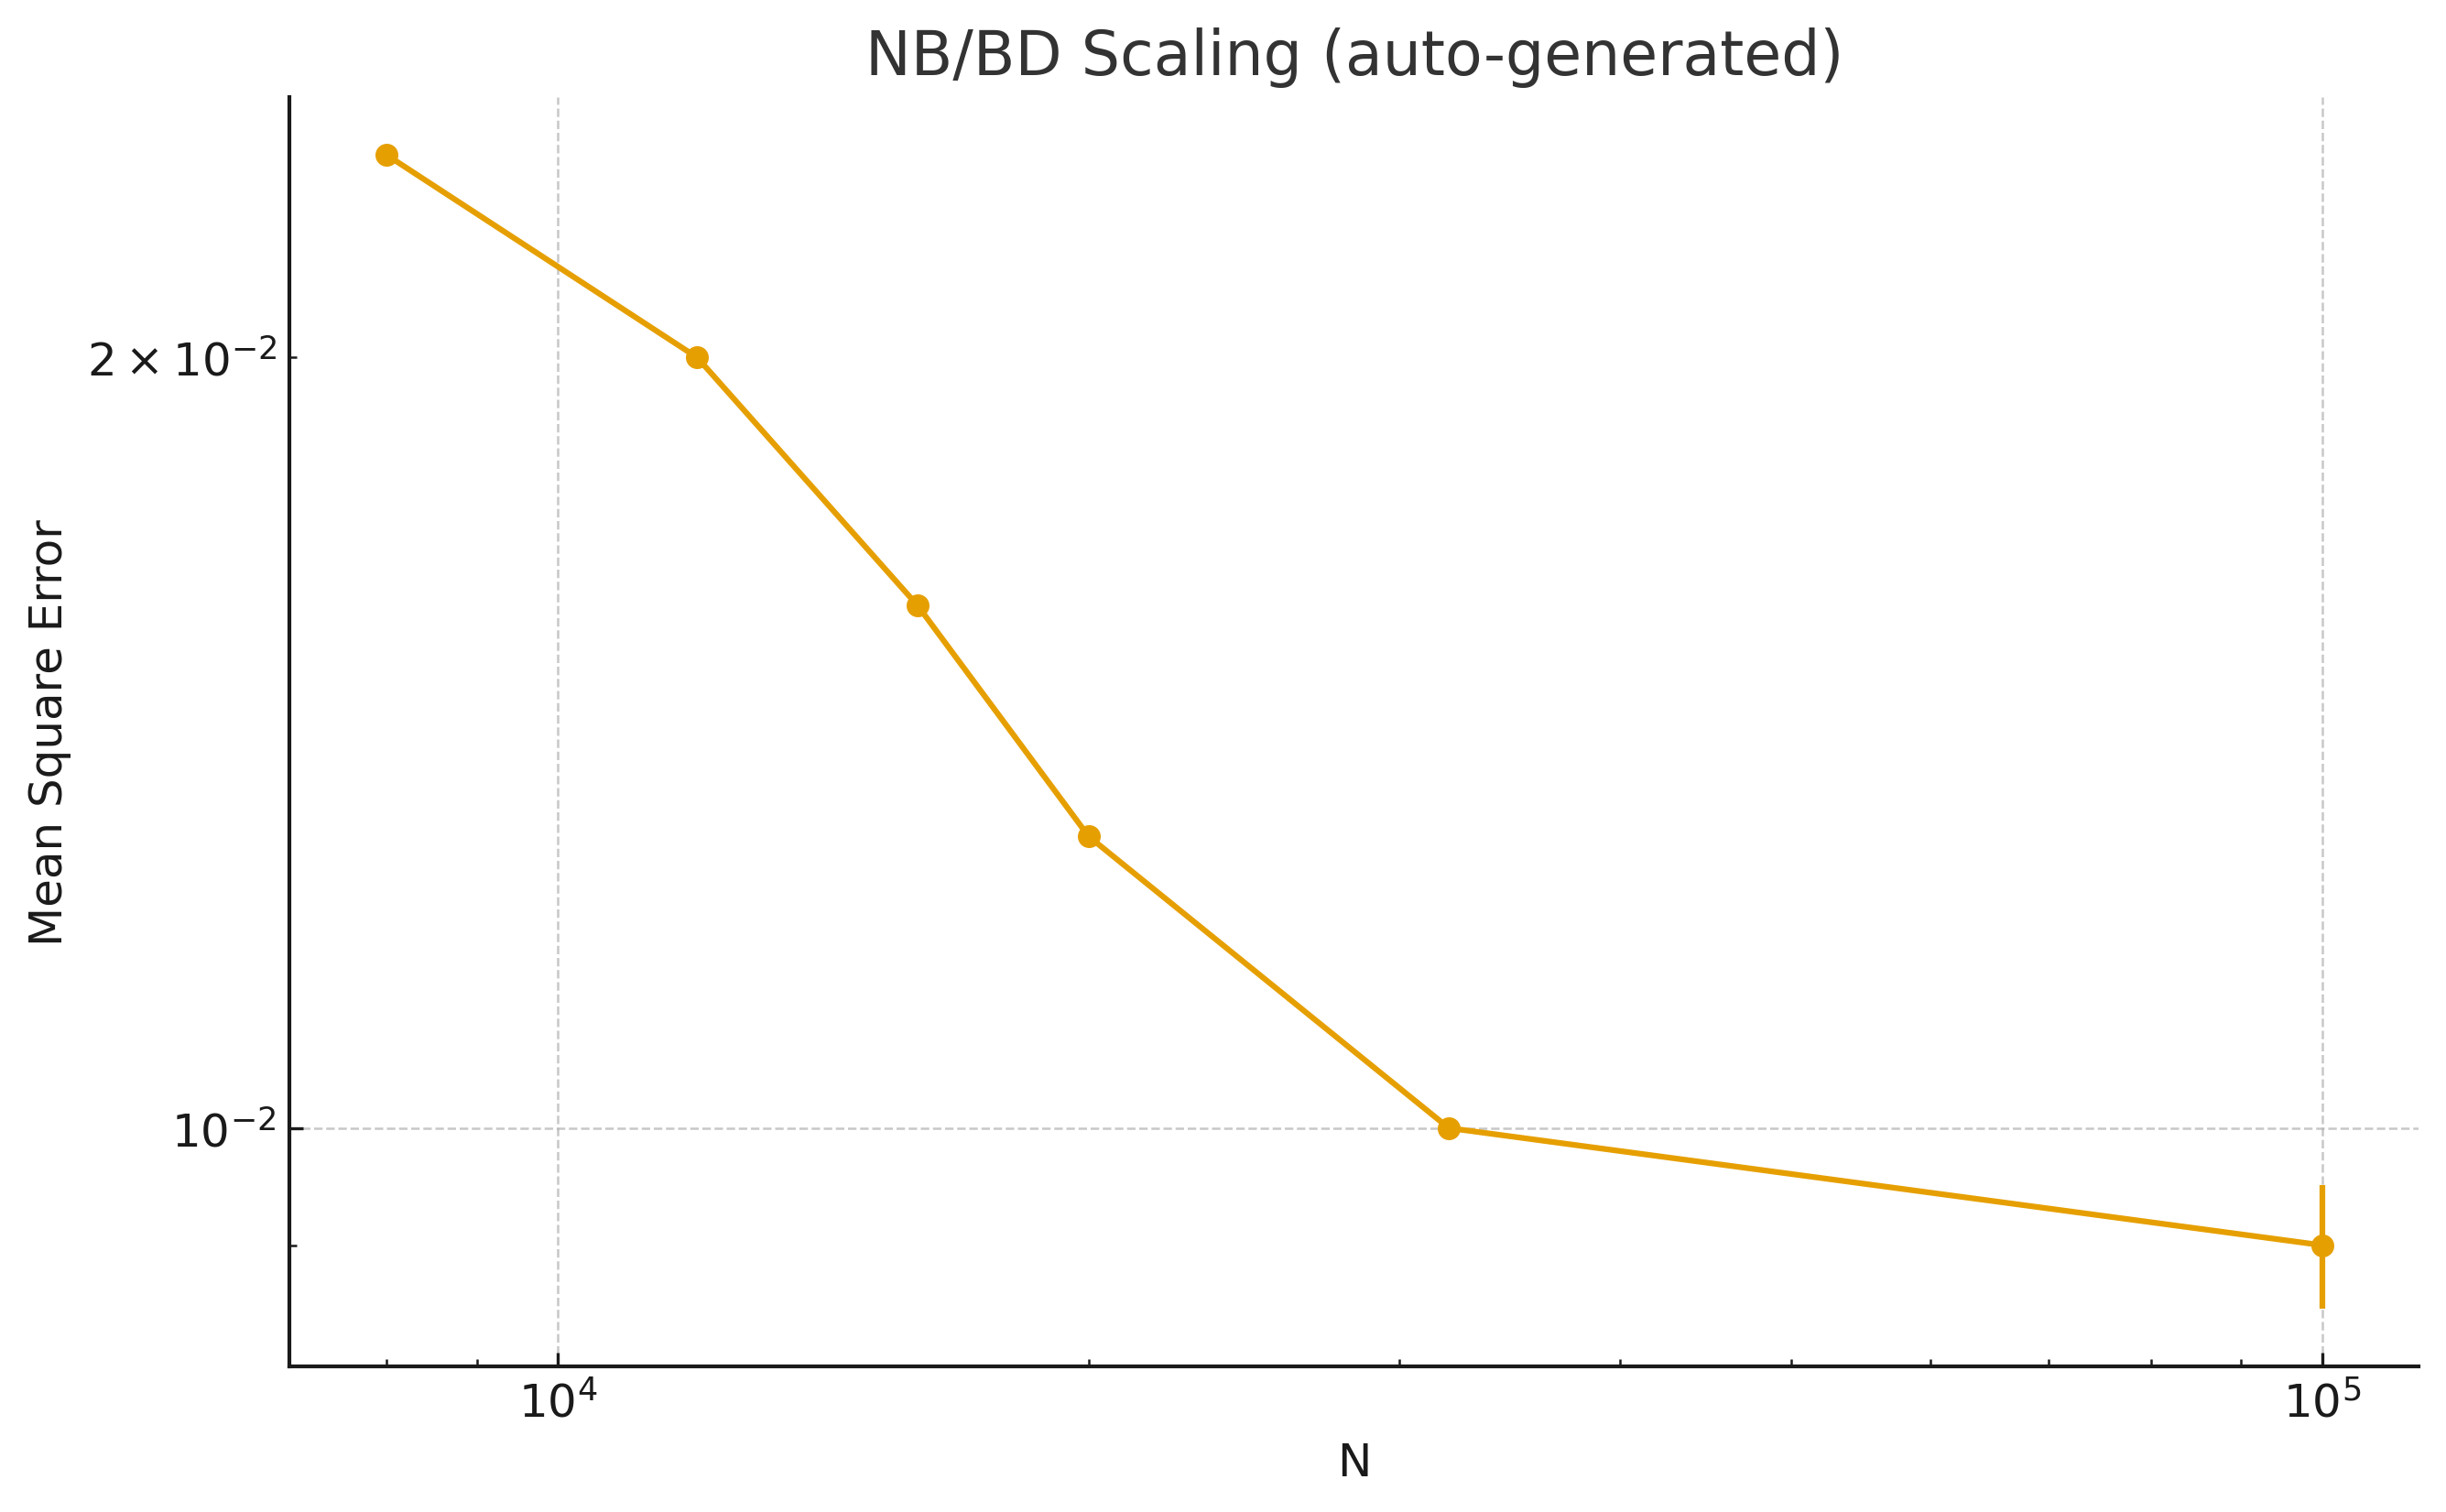
\includegraphics[width=0.8\linewidth]{figures/nbbd_scaling.png}
\caption{NB/BD mean-square vs $N$; log-log axes. Error bars where available.}
\end{figure}

\begin{thebibliography}{9}
\bibitem{baezduarte2003}
L.~B\'aez-Duarte,
\emph{A strengthening of the Nyman--Beurling criterion for the Riemann Hypothesis},
Atti Accad. Naz. Lincei Cl. Sci. Fis. Mat. Natur. Rend. Lincei (9) Mat. Appl. \textbf{14} (2003), 5--11.
\bibitem{conrey2003}
J.~B. Conrey,
\emph{The Riemann Hypothesis},
Notices Amer. Math. Soc. \textbf{50} (2003), no.~3, 341--353.
\bibitem{titchmarsh1986}
E.~C. Titchmarsh (rev. D.~R. Heath-Brown),
\emph{The Theory of the Riemann Zeta-Function}, 2nd ed., OUP, 1986.
\bibitem{montvau2007}
H.~L. Montgomery and R.~C. Vaughan,
\emph{Multiplicative Number Theory I}, CUP, 2007.
\end{thebibliography}

\end{document}
